\lab{Applications}{Job Search Model}{Job Search Model}

\section*{Discrete Choice (Threshold) Problems}\label{SecDiscrChoice}

One powerful application of dynamic programming that illustrates its versatility as a dynamic solution method is to models that have both continuous and discrete state variables. These models are sometimes referred to as discrete choice problems or optimal stopping problems.  Examples include models of employment that involve both the choice of whether to work and how much to work, models of firm entry and exit that involve the choice of both whether to produce and how much to produce, and models of marriage that involve the choice of whether to date (get married or keep dating) and how much to date.

In this problem set, we follow a simple version of a standard job search model.  Assume that workers are infinitely lived. Let the value of entering a period with most recent wage $w$, current job offer wage $w'$, and employment status $s$ be given by the following value function,
\begin{equation}\label{EqV}
   V(w,w',s) = \begin{cases}
                  V^E(w)    \quad&\text{if}\quad s = E \\
                  V^U(w,w') \quad&\text{if}\quad s = U \\
               \end{cases}
\end{equation}
where employment status is a binary variable $s=\{E,U\}$; a person can be either employed or unemployed.

If an individual's job status is employed ($s = E$) in a given period, then expected utility is the utility of consumption in the current period plus the discounted expected value of the entering the next period with wage $w$, job offer wage $w''$, and employment status $s'$.
\begin{equation}\label{EqVe1}
   V^E(w) = u(w) + \beta E_{w'',s'}V(w,w'',s')
\end{equation}
Here we assume that individuals spend all of their earnings each period so that utility from the consumption in the current period is $u(w)$.  The discount factor is $\beta$.  The next periods wage, $w''$, and job offer, $s'$, are unknown and we consider them as random variables.  Consequently, the expectations operator $E_{w'',s'}$ is over the job offer wage, and employment status in the next period, and next period's value function is simply \eqref{EqV} with the future value of employment status $s'$.

The joint probability distribution over $w''$ and $s'$ is characterized in the following simple way. If the worker stays employed in the next period $s' = E$, then next period's wage equals the current period's wage. If the worker becomes unemployed in the next period $s' = U$, then the worker's unemployment benefits will be a percentage of his current wage $\alpha w$. Any worker who is unemployed will receive one wage offer per period $w'$, which that worker will receive in the following period, drawn from the cumulative density function $F(w')$ or probability density function $f(w')$, which is independent of the worker's previous wage (for simplicity). Lastly, let $\gamma$ represent the probability that an employed worker becomes unemployed in the next period. So \eqref{EqVe1} can be rewritten in the following way.
\begin{equation}\label{EqVe2}
   V^E(w) = u(w) + \beta \Bigl[(1-\gamma)V^E(w) + \gamma E_{w''}V^U(w,w'')\Bigr]
\end{equation}

The value of being unemployed in a given period is a function of both the wage at the most recent job $w$ as well as the wage of the current job offer $w'$,
\begin{equation}\label{EqVu}
   V^U(w,w') = u(\alpha w) + \beta\max_{s'\in\{E,U\}}\Bigl\{V^E(w'),E_{w''}\left[V^U(w,w'')\right]\Bigr\}
\end{equation}
where $\alpha\in(0,1)$ is the fraction of the worker's previous wage paid in unemployment insurance benefits. The maximization in \eqref{EqVu} reflects the decision of whether to accept the current job offer or remain unemployed for another period.  It is only in the unemployed state $s=U$ in which the worker makes a decision. Once the job offer ($w'$) is received, the worker can choose whether to accept or reject the offer. The expectation in \eqref{EqVu} is, therefore, not over $w'$ but over the possible job offers in the following period, $w''$; if the worker chooses to reject the current job offer, then $s' = U$.

The policy function for the decision of the unemployed worker whether to accept a job $s'=E$ or whether to reject a job $s'=U$ will be a function of both the amount of the most recent wage $w$ and the amount of the current job offer: $s' = \psi(w,w')$. These discrete choice problems are often called threshold problems because the policy choice depends on whether the state variable is greater than or less than some threshold level. That is, an unemployed worker will accept a job if and only if the offer wage is above some set amount. In the labor search model, the threshold level is called the ``reservation wage'' $w_R'$. The reservation wage $w_R'$ is defined as the wage offer such that the worker is indifferent between accepting the job $s' = E$ and staying unemployed $s' = U$.
\begin{equation}\label{EqWR}
   w_R' \equiv w': V^E(w') = E_{w''}\left[V^U(w,w'')\right]
\end{equation}
Note that the reservation wage $w_R'$ is a function of the wage at the most recent job $w$ (if you have higher unemployment benefits you will wait for a higher job offer). The policy function will then take the form of accepting the job if $w' \geq w_R'$ or rejecting the job offer and stay unemployed if $w' < w_R'$.  Figure \ref{fig:disc_policy} shows an example of the discrete policy function.
\begin{equation}\label{EqSprime}
   s' = \psi(w,w') = \begin{cases}
                      E \quad\text{if}\quad w' \geq w_R' \\
                      U \quad\text{if}\quad w' < w_R'
                   \end{cases}
\end{equation}

\begin{figure}
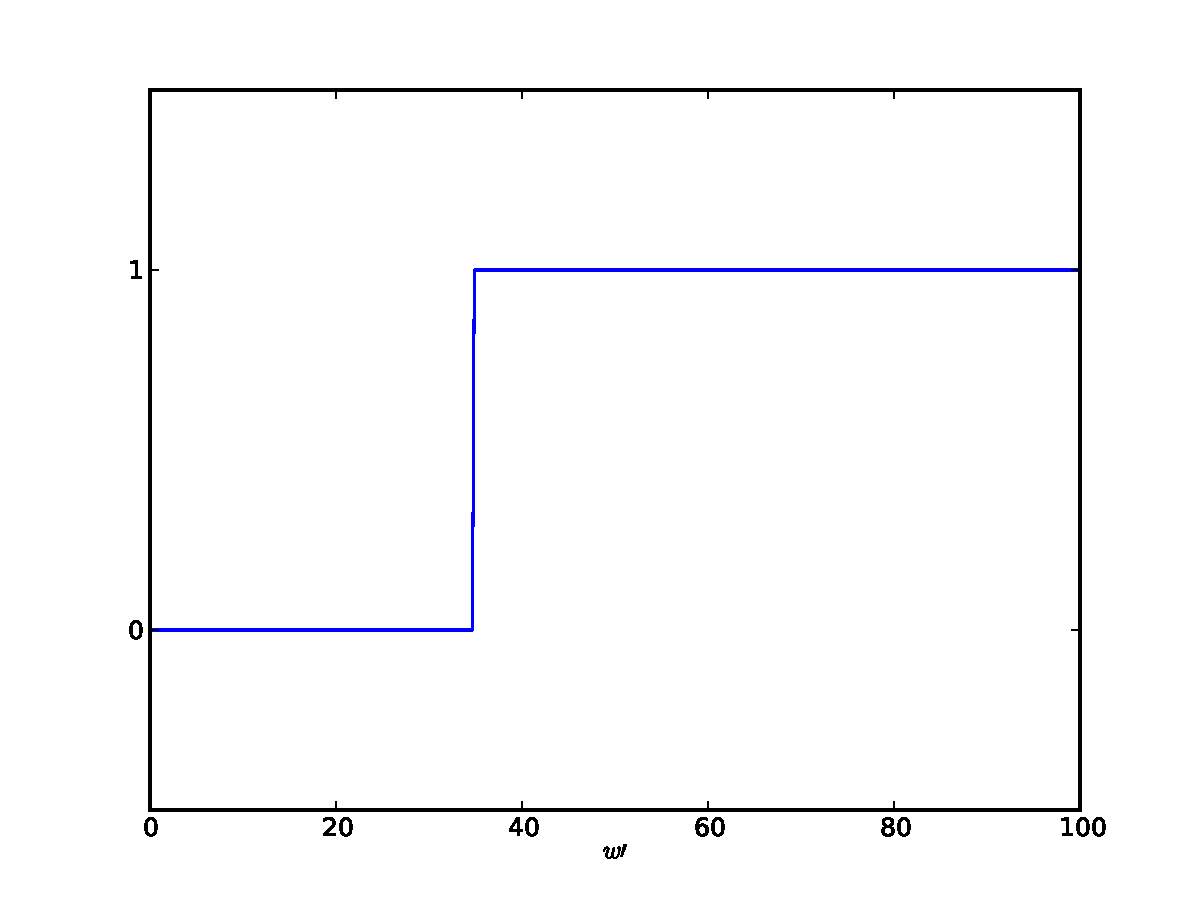
\includegraphics[width=\textwidth]{disc_policy.pdf}
\caption{Here is the policy function for fixed $w = 50$.  Numerically we let 0 represent unemployment, $U$, and 1 represent employment, $E$.  Thus we see that an individual will choose to take a new job, given their old wage was 50, at a wage of roughly 35.  Thus for a previous wage of 50, we say the reservation wage is 35.}
\label{fig:disc_policy}
\end{figure}

In summary, the labor search discrete choice problem is characterized by the value functions \eqref{EqV}, \eqref{EqVe2}, and \eqref{EqVu}, the reservation wage \eqref{EqWR}, and the policy function \eqref{EqSprime}. Because wage offers are distributed according to the cdf $F(w')$ and because the policy function takes the form of \eqref{EqSprime}, the probability that the unemployed worker receives a wage offer that he will reject is $F(w_R')$ and the probability that he receives a wage offer that he will accept is $1 - F(w_R')$. Just like the continuous choice cake eating problems, this problem can be solved by value function, policy function, or modified policy function iteration.

The value function iteration solution method for the equilibrium in the labor search problem is analogous to the value function iteration from the previous labs. The only difference is that two value functions ($V^E$ and $V^U$) must converge to a fixed point in this problem instead of just one value function converging in the previous problems.  Although there are two value functions to consider, there is only one policy function since decisions are only made in the unemployed state.  Thus there is only one policy function to iterate on in the case of policy or modified policy iteration.

Assume that the probability of becoming unemployed in a given period is $\gamma = 0.10$, the fraction of wages paid in unemployment benefits is $\alpha = 0.5$, and the discount factor is $\beta = 0.9$. Assume that the log of wage offers are distributed normally.  We then say that offers are distributed lognormally and write $w'\sim \text{LogN}(\mu,\sigma)$.  We let $m=20$ be the mean wage, $v=400$ be the variance of the wage.  Often lognormal distributions are reported with the mean and variance of $\log(w')$ which is distributed normally, but for simplicity you will not have to deal with that here. This is a convenient choice for the distribution of wage offers.  Among other things, it guarantees that wage offers will be positive.  Denote the cdf of the lognormal distribution as $F(w')$ and the pdf of the distribution as $f(w')$.

\begin{problem}
\begin{enumerate}

   \item Approximate the support of $w\in(0,\infty)$ by generating a column vector of possible values for $w$. Let the maximum value be $w_{max} = 100$, let the minimum value be $w_{min} = 0$, and let the number of equally spaced points in the vector be $N = 500$. Let the wage of a job offer in any period be lognormally distributed with mean job offer of $m=20$ and variance $v =200$.  Generate the discrete approximation of the lognormal probability density function $f(w')$ using the function defined in discretelognorm.py which is provided.  As arguments, it takes the points where the approximation is needed (w), along with the mean and variance so that it can be called as

\begin{lstlisting}
f = discretelognorm(w,m,v)
\end{lstlisting}

    Then the $n$th entry of $f$ represents the probability that the job offer in the next period equals the $n$th entry of $w$, $\text{Pr}(w' = w_n)$.

   \item Solve for the equilibrium optimal policy function $s' = \psi(w,w')$ by value function iteration.  In this case we iterate on both value functions $V^E$ and $V^U$ each time through the loop.  In order to compute the expected value of $V^U$, just matrix multiply $V^U$ and $f$. Remember, the policy function $\psi(w,w')$ gives the choice of whether to accept the job offer if unemployed with a given previous wage and current job offer.  Thus it will be a vector of length $N$ of zeros and ones.  Again, use a tolerance level of $10^{-9}$ and require that both value functions must converge (compute a delta for each and iterate until both are less than $10^{-9}$).

   \item Compute the reservation wage $w_R'$ as a function of the current wage $w$.  The reservation wage is the value of $w$ where the policy function changes from zeros to ones (the optimal choice changes from remaining unemployed to accepting the job offer).  If psi is an $N\times N$ matrix representing the policy function, the reservation wage wr could be computed as follows
   \begin{lstlisting}
    wr_ind = sp.argmin(sp.diff(psi), axis = 1)
    wr = w[wr_ind]
   \end{lstlisting}
	where the rows of psi correspond to values of $w$ and the columns correspond to values of $w'$.

   \item Plot the equilibrium reservation wage $w_R'$ of the converged problem as a function of the current wage $w$ with the current wage on the $x$-axis and the reservation wage $w_R'$ on the $y$-axis. This is the most common way to plot discrete choice policy functions. The reservation wage represents the wage that makes the unemployed worker indifferent between taking a job offer and rejecting it. So any wage above the reservation wage line represents $s' = E$ and any wage below the reservation wage line represents $s' = U$.

\end{enumerate}
\end{problem}

In the previous problem, it was necessary to iterate on two value functions.  Consequently the convergence is relatively slow.  Thus the gains by using modified policy function iteration are considerable.

\begin{problem}
Solve the same problem, this time using modified policy function iteration with $m=15$ value function iterations within each policy iteration.  Roughly, you can structure your code as follows:

\begin{enumerate}
	\item Initialize $w$,$u(\alpha w)$, $f$, $\gamma$, and $\beta$.  This should be the same as the previous problem.
	
	\item	Initialize $V^E$, $V^U$, and $E[V^U]$ to zeros.  Then begin the while loop.
	
	\item Inside the while loop update the policy function.  It is determined as
	\begin{equation}
		\psi (w,w') = \text{argmax} \left\{ V^E(w'), E_{w''}[V^U(w,w'')]\right\}
	\end{equation}
	
	\item Begin a for loop to iterate on the value functions.  Unlike in the previous algorithms lab, there is no $Q$ matrix in this case.  Given the previous iteration's value functions, updating $V^E$ should be simple because it does not depend directly on the policy function.
	
	To iterate on $V^U$, we need to compute $V^U$ given the current policy.  The policy determines the maximization in equation \eqref{EqVu}.  One way to compute the max is to use $\psi$ as a mask.  $V^U$ could be computed as follows:
	
\begin{lstlisting}
arg1 = sp.repeat(sp.transpose(VE),N,0)*psiprime
arg2 = sp.repeat(EVU,N,1)*(1-psiprime)
arg = arg1+arg2
VUprime = alpha_util_grid + beta*arg
\end{lstlisting}	

	where the ordering is such that $1$ corresponds to the state $E$ and $0$ corresponds to the state $U$.
	
	\item Compute the $\delta$'s.
	
	\item After the while loop you should compute the reservation wage and plot it.
\end{enumerate}
\end{problem}

\begin{problem}
How many iterations did value function iteration take?
How many iterations did modified policy function iteration take?
Which was faster?
\end{problem} 